\section{The constant \texorpdfstring{$A(p)$}{A(p)}}
\label{a:sec:Ap}

The conditioning argument in \ChM reduces the late-time law to the single constant
\begin{equation}
\label{a:eq:Apdef}
A(p) = \lim_{n\to\infty}\frac{S_n}{(2p)^n},
\qquad p\in[0,\tfrac12),
\end{equation}
whose reciprocal is the quasi-stationary mean.  The results below are original to
this thesis.  They are developed here because the preceding quasi-stationary
analysis reduces to $A(p)$, while later chapters repeatedly use the resulting
numerical scheme.

Away from criticality, approximate values are readily obtained by iterating
$S_{n+1}=2pS_n-pS_n^2$ until the ratio $S_n/(2p)^n$ stabilises.  Repeating the
calculation over a range of $p$ traces the discrete curve discussed in
\cref{a:sec:compare}.  The method becomes impractical as $p\to\tfrac12^-$,
however, because the number of generations required for stabilisation grows
without bound.

No formula in elementary functions is known for $A(p)$.  The analysis begins with
an exact infinite product (\cref{a:sec:product}) and an exact series whose
two-sided bounds locate $A(p)$ relative to the continuous-time constant
\cref{a:eq:Acts} (\cref{a:sec:Abounds}).  The series then yields the near-critical
asymptotic $A(p)\sim2(1-2p)$ (\cref{a:sec:A-near-critical}) and resolves the
apparent discrepancy between the discrete and continuous curves
(\cref{a:sec:compare}).  Against that analytic background, the symbolic-regression
searches in \cref{a:sec:GA} become diagnostic rather than merely negative, and the
dynamical argument in \cref{a:sec:koenigs} explains the obstruction they encounter.
The practical consequences are collected in \cref{a:sec:practical}.

\subsection{An infinite-product representation}
\label{a:sec:product}

Take the nonlinear map for the survival probability,
\begin{equation*}
S_{n+1} = 2pS_n - pS_n^2,\qquad S_0=1,
\end{equation*}
and substitute $S_n = 2w_n$. This gives
\begin{equation}
\label{a:eq:logistic}
w_{n+1} = 2p\,w_n(1-w_n) = r\,w_n(1-w_n),
\qquad r = 2p,\quad w_0 = \tfrac12 ,
\end{equation}
which is the logistic map.  Across the full range $0\leq r\leq4$, this family
exhibits the period-doubling route to chaos shown in
\cref{a:fig:period_double}.  Subcritical branching occupies only the interval
$r\in[0,1)$, where the origin is globally attracting.  The fact that even this
dynamically simple regime carries a closed-form obstruction is developed in
\cref{a:sec:koenigs}.

\begin{figure}[ht]
    \centering
    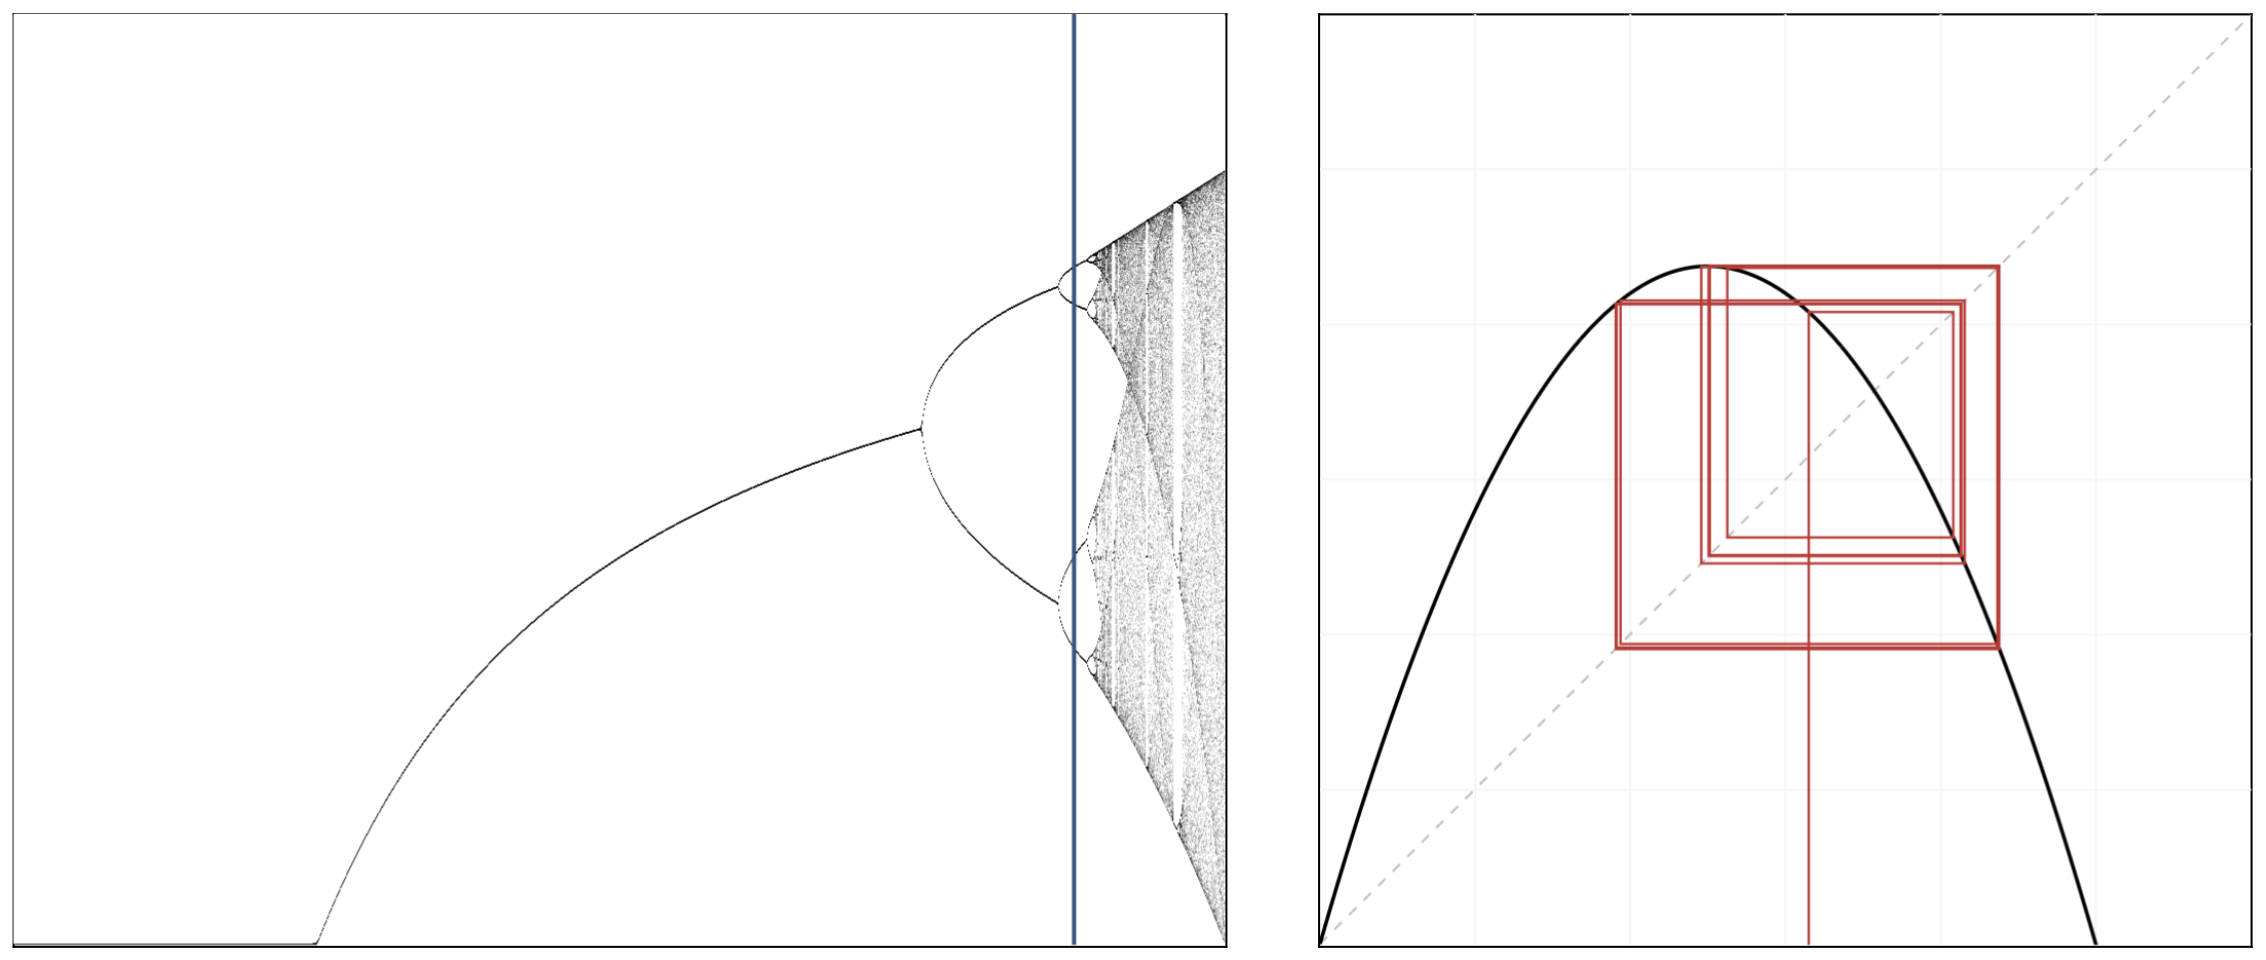
\includegraphics[width=0.86\textwidth]{figures/IMG_ch3/period_double.png}
    \caption{Bifurcation diagram of the logistic map $w\mapsto rw(1-w)$, showing
    the period doubling of stable states and the onset of chaos. The blue sample
    line on the left is at $r=3.5255$; the right-hand plot shows a trajectory of
    the map at the same $r$. The regime relevant to subcritical branching is
    $r=2p\in[0,1)$, off the left-hand edge of this diagram, where the dynamics are
    as simple as they can be.}
    \label{a:fig:period_double}
\end{figure}

In terms of $w$, \cref{a:eq:Apdef} reads
\begin{equation}
\label{a:eq:Aw}
A(p) = \lim_{n\to\infty}\frac{S_n}{(2p)^n} = 2\lim_{n\to\infty}\frac{w_n}{r^n} .
\end{equation}
The limit in \cref{a:eq:Aw} can be reorganised as a telescoping product.  For any
sequence,
\begin{equation*}
x_n = x_0\lrb{\frac{x_1}{x_0}}\lrb{\frac{x_2}{x_1}}\cdots\lrb{\frac{x_n}{x_{n-1}}}
= x_0\prod_{k=0}^{n-1}\frac{x_{k+1}}{x_k},
\qquad\text{so}\qquad
\lim_{n\to\infty}x_n = x_0\prod_{k=0}^{\infty}\frac{x_{k+1}}{x_k},
\end{equation*}
Applying this identity to $x_n=w_n/r^n$ gives a ratio in which the multiplier
cancels:
\begin{equation*}
\frac{x_{k+1}}{x_k}
= \frac{w_{k+1}}{w_k}\cdot\frac1r
= \frac{rw_k(1-w_k)}{w_k}\cdot\frac1r
= 1-w_k .
\end{equation*}
Hence, with $x_0 = w_0 = \tfrac12$ and $A(p) = 2\lim_n x_n$,
\begin{equation*}
A(p) = 2\cdot\tfrac12\prod_{k=0}^{\infty}(1-w_k) = \prod_{k=0}^{\infty}(1-w_k),
\end{equation*}
and pulling out the factor $1-w_0=\tfrac12$,
\begin{equation}
\label{a:eq:prodFormula}
A(p) = \frac12\prod_{k=1}^{\infty}(1-w_k)
= \frac12\prod_{k=1}^{\infty}\lrb{1-\frac{S_k}{2}} .
\end{equation}

\subsubsection*{Convergence}

For $0<w_k<1$, the product $\prod_{k\ge1}(1-w_k)$ converges to a strictly
positive limit if and only if $\sum_{k\ge1}w_k<\infty$.  In the present regime,
\cref{a:eq:logistic} gives $w_{n+1}<rw_n$ for $0<r<1$, and induction therefore
yields $w_n\leq w_0r^n$.  This geometric bound is summable, so the product
converges to a positive finite value.  It follows directly that the limit in
\cref{a:eq:Apdef} exists and that $0<A(p)<\tfrac12$ for
$p\in(0,\tfrac12)$.

\subsubsection*{Is this an advance?}

The advance is modest but useful.  Equation \cref{a:eq:prodFormula} is exact, and
its partial products decrease monotonically, so every truncation gives a rigorous
upper bound on $A(p)$; the raw ratio $S_n/(2p)^n$ offers no such bound.  Computing
the factors still requires iteration of the nonlinear map, however, and therefore
does not remove the near-critical cost.  The greater value of the product is that
it opens a route to the sharper series representation below.

\subsection{An exact series and two-sided bounds}
\label{a:sec:Abounds}

The same recursion also produces a telescoping sum, which exposes more of the
dependence on $p$.  Write $r=2p$ and factorise the recurrence as
\begin{equation*}
S_{n+1} = rS_n\lrb{1-\frac{S_n}{2}} .
\end{equation*}
Define $v_n = r^n/S_n$, so that $v_n\to1/A(p)$ by \cref{a:eq:Apdef}. Then
\begin{equation*}
v_{n+1}-v_n
= \frac{r^{n+1}}{rS_n\lrb{1-\frac{S_n}{2}}} - \frac{r^n}{S_n}
= \frac{r^n}{S_n}\lrbs{\frac{1}{1-\frac{S_n}{2}}-1}
= \frac{r^n}{S_n}\cdot\frac{S_n/2}{1-\frac{S_n}{2}}
= \frac{r^n}{2-S_n} .
\end{equation*}
Summing from $v_0 = 1/S_0 = 1$ gives an exact representation of the
quasi-stationary mean.

\begin{proposition}[Series representation]
\label{a:prop:series}
For $p\in[0,\tfrac12)$, with $S_n$ generated by \cref{a:eq:SnIter},
\begin{equation}
\label{a:eq:Aseries}
\frac{1}{A(p)} = 1 + \sum_{n=0}^{\infty}\frac{(2p)^n}{2-S_n} .
\end{equation}
\end{proposition}

\noindent
Unlike the product, this representation isolates the geometric decay in a factor
independent of the nonlinear dynamics; all nonlinearity is confined to the bounded
denominator $2-S_n$.  Since $S_n\in(0,1]$, that denominator lies in $[1,2)$.
Bounding it at these two extremes and summing the resulting geometric series gives
the following estimates.

\begin{proposition}[Two-sided bounds]
\label{a:prop:bounds}
With $\varepsilon=1-2p$ as in \cref{a:eq:epsdef}, for $p\in(0,\tfrac12)$,
\begin{equation}
\label{a:eq:Abounds}
\frac{\varepsilon}{1+\varepsilon} \;<\; A(p) \;<\; \frac{2\varepsilon}{1+2\varepsilon},
\end{equation}
that is,
\begin{equation}
\label{a:eq:Aboundsexplicit}
\frac{1-2p}{2(1-p)} \;<\; A(p) \;<\; \frac{2(1-2p)}{3-4p} .
\end{equation}
The lower bound is exactly half the continuous-time constant \cref{a:eq:Acts}:
\begin{equation}
\label{a:eq:halfAc}
A(p) > \tfrac12\Ac(p) .
\end{equation}
\end{proposition}

\begin{proof}
Since $0<S_n\le1$ for all $n$ we have $1\le2-S_n<2$, and hence
$\tfrac12r^n < r^n/(2-S_n)\le r^n$, with equality on the right only at $n=0$, where
$S_0=1$. Summing over $n\ge0$ and using $\sum_nr^n = 1/(1-r) = 1/\varepsilon$,
\begin{equation*}
1+\frac{1}{2\varepsilon} \;<\; \frac{1}{A(p)} \;<\; 1+\frac{1}{\varepsilon},
\end{equation*}
and inverting gives \cref{a:eq:Abounds}. Substituting $\varepsilon=1-2p$ gives
\cref{a:eq:Aboundsexplicit}, whose lower bound is
$(1-2p)/\bigl(2(1-p)\bigr) = \tfrac12\Ac(p)$ by \cref{a:eq:Acts}.
\end{proof}

The two endpoints of \cref{a:prop:bounds} account for the shape of the discrete
curve.  As $p\to0$, one has $\varepsilon\to1$ and the lower bound tends to
$\tfrac12$.  The parity bound below gives $A(p)\leq\tfrac12$, so the lower bound
is asymptotically attained and $A(0^+)=\tfrac12$.  At the other endpoint,
$p\to\tfrac12^-$, the lower bound is asymptotic to $\varepsilon$ and the upper
bound to $2\varepsilon$; \cref{a:sec:A-near-critical} shows that $A(p)$ approaches
the upper scale.  The constant therefore moves from one bounding regime to the
other across the interval, which rules out any constant rescaling of $\Ac$.

\begin{proposition}[Parity bound]
\label{a:prop:parity}
For the binary Galton--Watson process started from a single individual,
$A(p)\le\tfrac12$ for all $p\in[0,\tfrac12)$, with equality approached as $p\to0$.
\end{proposition}

\begin{proof}
Every individual leaves either $0$ or $2$ offspring, so $Z_n$ is even for every
$n\ge1$. Conditional on survival, therefore, $Z_n\ge2$, and hence
$\ex{Z_n\mid Z_n>0}\ge2$ for all $n\ge1$. Letting $n\to\infty$ and using
\cref{a:eq:qsmean} gives $1/A(p)\ge2$. As $p\to0$ the conditional population is $2$
with probability tending to one, so the bound is attained in the limit.
\end{proof}

\begin{table}[ht]
\centering
\caption{The constant $A(p)$ computed from \cref{a:eq:prodFormula} in
$60$-digit arithmetic, together with the bounds of \cref{a:prop:bounds} and the
near-critical asymptotic $2(1-2p)$ from \cref{a:sec:A-near-critical}.  The bounds
are widest in the middle of the interval and tighten at its ends: at $p=0.05$ the
lower bound is within $3\%$ of $A$, whereas at $p=0.4999$ the upper bound is within
$0.1\%$.  The final columns give the quasi-stationary mean and the number of
product factors required for full precision, which is the computational cost
addressed in \cref{a:sec:practical}.}
\label{a:tab:Avals}
\begin{tabular}{ccccccr}
\toprule
$p$ & $\tfrac12\Ac(p)$ & $A(p)$ & $\dfrac{2(1-2p)}{3-4p}$ & $2(1-2p)$ & $1/A(p)$ & iterations\\
\midrule
0.05   & 0.473684 & 0.486180 & 0.642857 & 1.800000 & 2.0568 & 45 \\
0.1    & 0.444444 & 0.469382 & 0.615385 & 1.600000 & 2.1305 & 64 \\
0.2    & 0.375000 & 0.423895 & 0.545455 & 1.200000 & 2.3591 & 113 \\
0.3    & 0.285714 & 0.353967 & 0.444444 & 0.800000 & 2.8251 & 201 \\
0.4    & 0.166667 & 0.237647 & 0.285714 & 0.400000 & 4.2079 & 458 \\
0.45   & 0.090909 & 0.145069 & 0.166667 & 0.200000 & 6.8933 & 966 \\
0.48   & 0.038462 & 0.068011 & 0.074074 & 0.080000 & 14.7036 & 2\,473 \\
0.49   & 0.019608 & 0.036395 & 0.038462 & 0.040000 & 27.4764 & 4\,965 \\
0.499  & 0.001996 & 0.003944 & 0.003984 & 0.004000 & 253.519 & 48\,992 \\
0.4999 & 0.000200 & 0.000399 & 0.000400 & 0.000400 & 2504.65 & 478\,905 \\
\bottomrule
\end{tabular}
\end{table}
